%!TEX TS-program = xelatex
%!TEX encoding = UTF-8 Unicode


\documentclass[12pt]{extarticle}
% extarticle is like article but can handle 8pt, 9pt, 10pt, 11pt, 12pt, 14pt, 17pt, and 20pt text

\def \ititle {Philosophical Psychology}

\def \isubtitle {Lecture 13}

\def \iauthor {Stephen A. Butterfill}
\def \iemail{s.butterfill@warwick.ac.uk}
\date{}

%for strikethrough
\usepackage[normalem]{ulem}

\input{$HOME/latex_imports/preamble_steve_handout}

%\bibpunct{}{}{,}{s}{}{,}  %use superscript TICS style bib
%remove hanging indent for TICS style bib
%TODO doesnt work
\setlength{\bibhang}{0em}
%\setlength{\bibsep}{0.5em}


%itemize bullet should be dash
\renewcommand{\labelitemi}{$-$}

\begin{document}

\begin{multicols*}{3}

\setlength\footnotesep{1em}


\bibliographystyle{newapa} %apalike

%\maketitle
%\tableofcontents




%---------------
%--- start paste


      
\def \ititle {13: Twin Interface Problems}
 
\begin{center}
 
{\Large
 
\textbf{\ititle}
 
}
 
 
 
\iemail %
 
\end{center}
 
 
 
\section{An Interface Problem}
 
Background assumptions
\begin{enumerate}
  \item Motor representations specify goals.
  \item Intentions specify goals.
  \item  Some actions involve both intention and motor representation.
  \item  Intention and motor representation are not inferentially integrated (because representational format?).
\end{enumerate}

Interface problem: How does it come about that intentions and motor representations
ever specify outcomes that non-accidentally match?

Two collections of outcomes, A and B, \emph{match} in a particular context just if, in that context,
either the occurrence of the A-outcomes would normally constitute or cause, at least partially, the
occurrence of the B-outcomes or vice versa. To illustrate, one way of matching is for the B-outcomes
to be the A-outcomes. Another way of matching is for the B-outcomes to stand to the A-outcomes as
elements of a more detailed plan stand to those of a less detailed one.

‘both mundane cases of action slips and pathological conditions, such as apraxia or anarchic hand
syndrome (AHS), illustrate the existence of an interface problem’ 
\citep[p.~7]{mylopoulos:2016_intentions}.
 
 
 
\section{Five Complications}

Complication 1: outcomes have a complex anatomy
comprising manipulation, target, form and more.

\begin{center}
    
  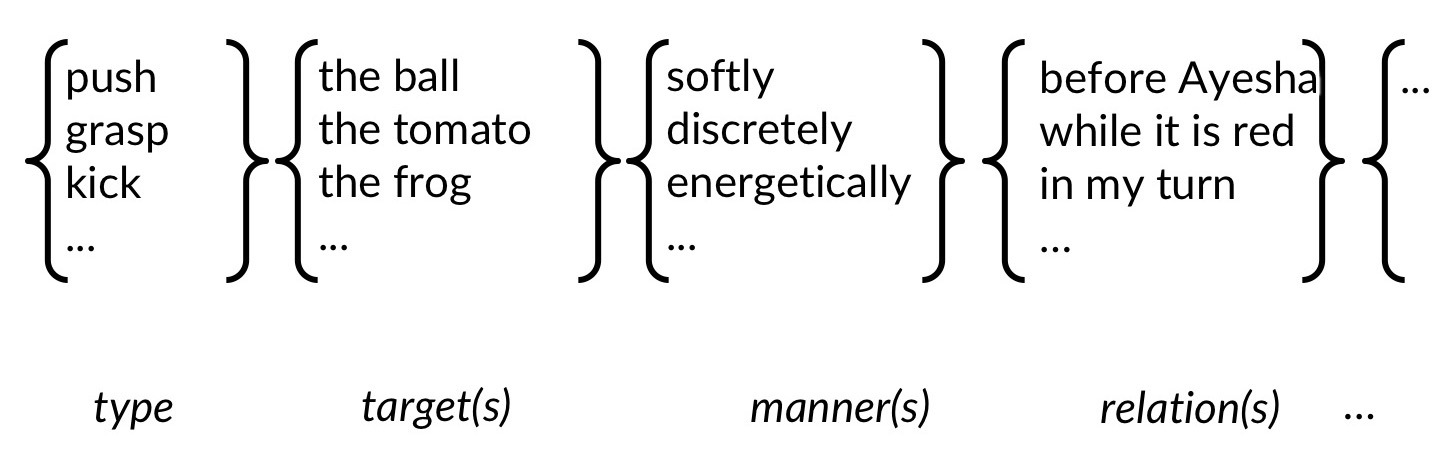
\includegraphics[scale=0.3]{fig/anatomy_of_a_goal.jpg}
  Anatomy of a Goal
  \end{center}
  
Complication 2: we can’t think of the interface problem merely as a way of intentions
setting problems to be solved by motor representations: instead, there may be multiple intentions
at different scales, and in some cases an intention may operate at a smaller scale than
a motor representation.

Complication 3: It’s ‘not just how motor representations are triggered by intentions, but how motor
representations’ sometimes nonaccidentally continue to match intentions as circumstances change in unforeseen ways ‘throughout
skill execution’
\citep[p.~19]{fridland:2016_skill}.
 
 Complication 4: there is a related developmental problem: What is the process by which humans acquire
 abilities to ensure that their intentions and motor representations sometimes nonaccidentally
 match?

 Complication 5: Imagination: intentions and motor representations can nonaccidentally match not only
 when we are acting but also when we are merely imagining acting.
 
\section{Mylopoulos and Pacherie’s Proposal}
 
‘As defined by Tutiya et al., an executable concept of a type of movement is a
representation, that could guide the formation of a volition, itself the proximal cause of
a corresponding movement. Possession of an executable concept of a type of movement thus
implies a capacity to form volitions that cause the production of movements that are
instances of that type.’
\citep[p.~7]{pacherie:2011_nonconceptual}
 
 
 
\section{A Puzzle about Thought, Experience and the Motoric}

1. In action observation, motor representations of outcomes  underpin goal-tracking, and
sometimes facilitate the identification of goals in thought.

2. So where motor representations influence a thought about an action being directed to a particular outcome, there is normally a motor representation of this outcome, or of a matching outcome.

3. But how could motor representations have content-respecting influences on thoughts given their inferential isolation?
 
  
  \section{The Twin Interface Problems}
 
  Interface Problem 1: intention -> motor representation
  \begin{quote}
  How could intentions have content-respecting influences on motor representations given their inferential isolation?
  \end{quote}
  
  Interface Problem 2: motor representation -> judgement
  
  
  \begin{quote}
    How could motor representations have content-respecting influences on thoughts given their inferential isolation?
    \end{quote}

\vfill
 

%--- end paste
%---------------

\footnotesize
\bibliography{$HOME/endnote/phd_biblio}

\end{multicols*}

\end{document}

    